%%%%%%%%%%%%%%%%%%%%%%%%%%%%%%%%%%%%%%%%%%%%%%%%%%%%%%%%%%%%%%%%%%%%%%%%
%    INSTITUTE OF PHYSICS PUBLISHING                                   %
%                                                                      %
%   `Preparing an article for publication in an Institute of Physics   %
%    Publishing journal using LaTeX'                                   %
%                                                                      %
%    LaTeX source code `ioplau2e.tex' used to generate `author         %
%    guidelines', the documentation explaining and demonstrating use   %
%    of the Institute of Physics Publishing LaTeX preprint files       %
%    `iopart.cls, iopart12.clo and iopart10.clo'.                      %
%                                                                      %
%    `ioplau2e.tex' itself uses LaTeX with `iopart.cls'                %
%                                                                      %
%%%%%%%%%%%%%%%%%%%%%%%%%%%%%%%%%%
%
%
% First we have a character check
%
% ! exclamation mark    " double quote
% # hash                ` opening quote (grave)
% & ampersand           ' closing quote (acute)
% $ dollar              % percent
% ( open parenthesis    ) close paren.
% - hyphen              = equals sign
% | vertical bar        ~ tilde
% @ at sign             _ underscore
% { open curly brace    } close curly
% [ open square         ] close square bracket
% + plus sign           ; semi-colon
% * asterisk            : colon
% < open angle bracket  > close angle
% , comma               . full stop
% ? question mark       / forward slash
% \ backslash           ^ circumflex
%
% ABCDEFGHIJKLMNOPQRSTUVWXYZ
% abcdefghijklmnopqrstuvwxyz
% 1234567890
%
%%%%%%%%%%%%%%%%%%%%%%%%%%%%%%%%%%%%%%%%%%%%%%%%%%%%%%%%%%%%%%%%%%%
%
\documentclass[10pt]{iopart}
%\newcommand{\gguide}{{\it Preparing graphics for IOP Publishing journals}}
%Uncomment next line if AMS fonts required
%\usepackage{iopams}
\usepackage{graphicx}
\usepackage{multirow}
\begin{document}

\title[Microwave induced defect engineering in SiC and GaAs]{Microwave induced defect engineering in SiC and GaAs}

\author{Oleg Olikh$^1$\footnote{Author to whom any correspondence should be addressed.}, Petro Lytvyn$^2$}

\address{$^1$Physics Faculty, Taras Shevchenko National University of Kyiv, Kyiv 01601, Ukraine}
\address{$^2$V. Lashkaryov Institute of Semiconductor Physics of NAS of Ukraine, Kyiv 03028, Ukraine}
\ead{olegolikh@knu.ua}
%\vspace{10pt}
%\begin{indented}
%\item[]August 2017
%\end{indented}

\begin{abstract}
The influence of microwave radiation (2.45~GHz, 1.5~W/cm$^2$, up to 80~s) on defects was studied in single crystals $n$-6H–SiC, $n$-GaAs and epi-GaAs.
The capture cross-section of charge carrier has been found to change
and defect complexes to be reconstructed due to the growing number of  interstitial atoms in the near surface layer.
The correlation between the changes in defect sub-system and deformation of the near surface layer is analyzed.
The possible mechanisms of the revealed effects are discussed.
\end{abstract}

%
% Uncomment for keywords
\vspace{2pc}
\noindent{\it Keywords}: microwave, defect, SiC, GaAs

% Uncomment for Submitted to journal title message
\submitto{\SST}
%
% Uncomment if a separate title page is required
%\maketitle

% For two-column output uncomment the next line and choose [10pt] rather than [12pt] in the \documentclass declaration
\ioptwocol
%


\section{Introduction}\label{sec:Int}

Microelectronics is a field of primary importance today, and the investigation of how semiconductors and their structure properties change under the action of various external factors has become one of the most important tasks in material science.
A great number of theoretical and experimental researches have been aimed at revealing degradation mechanisms in microelectronic devices and developing new technologies of their production.
The influence of certain factors, for example, radiation, has been studied quite well --- see, for instance, \cite{KozlovsEn,RadiationEffectsBook,DefByIon}.
At the same time, new agents begin to attract more attention, such as ultrasound loading (USL) \cite{Olikh2018JAP,Olikh2006TPL},
or microwave treatment (MWT) \cite{MW:Rev,ZOHM2000,BHUNIA1998,Bacherikov2003En,Pashkov1994En,
BoltovetsEn,Milenin1994En,BelyaevIntac,ASHKINADZE1996,ProcSPIE,Belyaev1998JTFEn,
Bacherikov2008En,Konakova2015En,Konakova2012FTPEn}.
As for MWT, the superhigh frequency (SHF) electromagnetic radiation has found a wide application due to its capability to heat solid bodies \cite{MW:Rev,ZOHM2000}.
This approach is peculiar because of its high efficiency, capability to increase the temperature
of a sample as a whole or at chosen locations with extremely high speeds of heating \cite{MW:Rev}.
As a result, MWT is widely used to synthesize various compounds, semiconducting compounds including \cite{MW:Rev,BHUNIA1998}.
However, this kind of external influence also causes the change in various characteristics of semiconductor materials and device structures.
For instance, it has been found that irradiation by  SHF causes the relaxation of internal stresses and modification of near surface regions
in GaAs and InP structures \cite{BoltovetsEn,Pashkov1994En,Milenin1994En,BelyaevIntac,ProcSPIE,Konakova2015En,Konakova2012FTPEn}, 
the leveling of surface microrelief in SiC/SiO$_2$ structures \cite{Bacherikov2003En},
redistribution of impurities \cite{Bacherikov2003En,Belyaev1998JTFEn,Konakova2015En}
and change in charge state in the complexes \cite{Milenin1994En} as well as generation of defects \cite{Belyaev1998JTFEn}.
One of the consequences the structure-admixture ordering  lead to is the decrease in the range of
Schottky diode parameter spread \cite{Milenin1994En,Belyaev1998JTFEn}.
Moreover, MWT has been found to induce changes in the properties of Ti, Gd and Er films deposited on silicon carbide \cite{Bacherikov2008En},
as well as reconstruction of GaAs photoluminescence spectra \cite{BelyaevIntac,ProcSPIE,Belyaev1998JTFEn},
the peculiarities of the effect being dependent both on the type of dopant and crystal structure orientation of the samples.
As a whole, these facts allow us to consider MWT as one of the most promising ways of modifying semiconductor devices.

On the other hand, it is of wide knowledge that the properties of semiconductor structures are determined very much by their defect subsystem.
In fact, the defects in SiC and GaAs are under active investigation up to now \cite{SiCDavid,SiCWei,GAPel2020,GASobolev2020}.
At the same time,
the more detailed information about how MWT influences deep center parameters is practically unknown.
The aim of our work is to investigate MWT impact on the parameters of deep centers located in the near surface region of $n$–-6H-–SiC and $n$-–GaAs single crystals,
as well as on  GaAs  epitaxial structures by means of acoustoelectric  transient spectroscopy.

\section{Experimental details}\label{sec:Exp}

It has been reported \cite{BoltovetsEn,Milenin1994En,BelyaevIntac,ASHKINADZE1996,ProcSPIE} that generally,
the MWT impact on semiconductor structures depends on many factors.
The main of them are the initial level of structural perfectness, conductivity, dielectric permittivity and structure topology.
In order to estimate how MWT affects the defect parameters we chose different samples in view of doping degree, initial level of residual mechanical stress as well as structure.
They were as follows.

\noindent
i)~Single crystal $n$--6$H$--SiC wafers, grown by Leli method and doped with nitrogen.
   The samples were:
    490~$\mu$m thick plates with dimensions $5\times10$~mm$^2$ and  carrier concentration $(3-6)\times10^{18}$~cm$^{-3}$
    (further on SIC1 and SIC2);
    and 460~$\mu$m thick wafer of the same dimensions with concentration of carriers $(1-3)\times10^{18}$~cm$^{-3}$ (SIC3).

\noindent
ii)~GaAs single crystal plates with thickness of 300~$\mu$m.
   The plates were (100) oriented, doped with tin, the concentration of electrons was $(1.5-2.5)\times10^{18}$~cm$^{-3}$
   for sample  GAS1 and $(3-5)\times10^{16}$~cm$^{-3}$ for sample GAS2.
   GAT denotation is used for wafer (111), which was doped by tellurium,  $n = (1-2)\times10^{18}$~cm$^{-3}$.

\noindent
iii)~Epitaxial $n$-$n^+$ structures of GaAs which were 300~$\mu$m thick single crystal substrates $n = 2 \times10^{18}$~cm$^{-3}$
   covered with 6~$\mu$m thick layer with carrier concentration $3.9\times10^{15}$~cm$^{-3}$
   (sample GAE1), $3.5\times10^{15}$~cm$^{-3}$ (GAE2),
   $5.0\times10^{15}$~cm$^{-3}$ (GAE3).
   The substrate and epitaxial layer were doped with tellurium.

\noindent
iv)~Epitaxial $n$-$n^+$-$n^{++}$ structures of GaAs:Te with a buffer layer.
 They were made from single crystal (100) substrate (300~$\mu$m, $n= 2\times10^{18}$~cm$^{-3}$)
  subsequently covered with 1~$\mu$m layer with $n=8\times10^{16}$~cm$^{-3}$ and
  2~$\mu$m layer with $n=7\times10^{15}$~cm$^{-3}$.
  Two samples (GAB1 and GAB) were cut from different wafers and used in the investigation.

Epitaxial systems were produced by the gas phase epitaxy technique.
The samples used in the experiment are categorized in \fref{figSamp_TAV}.

\begin{figure}
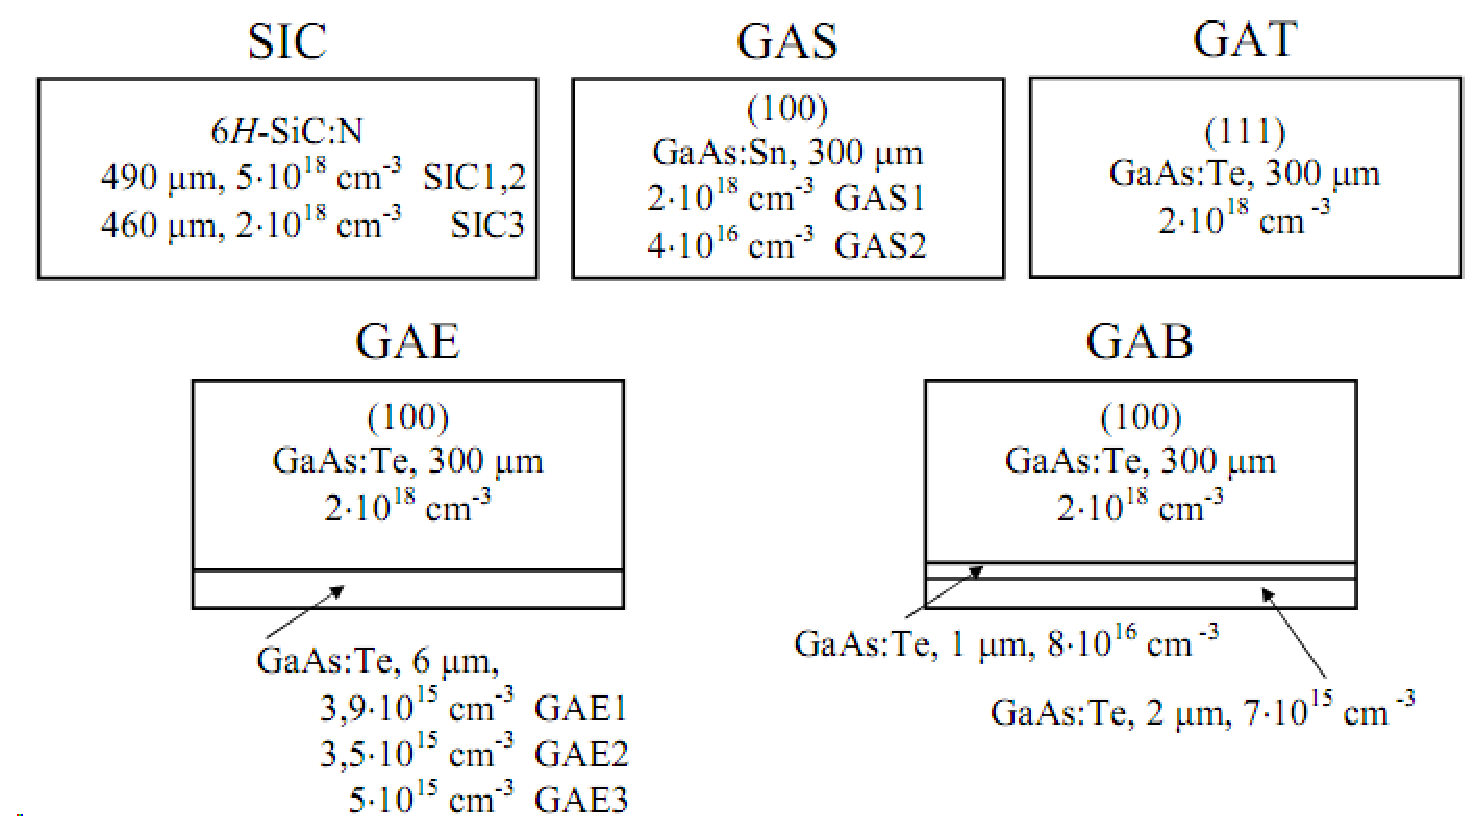
\includegraphics[width=0.5\textwidth]{Fig1}
\caption{\label{figSamp_TAV}
Structures for deep level investigations
}%
\end{figure}

MWT of the sample was carried out in free space at room temperature in the magnetron at the frequency of  $2.45$~GHz
and specific power $1.5$~W/cm$^{2}$.
The epitaxial structures were irradiated from the side of the epitaxial layer.
The total exposition time $t_\mathtt{MWT}$ varied in the range $20-80$~s for different samples.
To avoid essential heating, the maximum single irradiation exposure time was no more than  five seconds.


The parameters of deep centers, such as the efficient cross section of electron capture $\sigma_n$
and location of the center energy level with relation to conductivity band bottom $E_c-E_t$ were determined before and after MWT.
For this purpose, we used acoustoelectric transient spectroscopy \cite{OstrovPAN,OlikhSSC,PANnewEn,OstrovskiiSST}.
The method is schematically presented in \fref{figTAV}.
The samples were placed on the LiNbO$_3$ piezoelectric plate in which acoustic waves were excited as impulses.
After ultrasound impulse termination, the relaxation of transverse acoustoelectric voltage (TAV) takes place according to the law
\begin{equation}\label{eqVtav}
  V_\mathtt{TAV}(t)=V_{\mathtt{TAV},0}\exp(-t/\tau).
\end{equation}

\begin{figure}
\includegraphics[width=0.5\textwidth]{fig2}
\caption{\label{figTAV}
Scheme of TAV signal  measurements.
Time dependence of radio impulse $V_\mathtt{RF}$ of ultrasound excitation in piezoelectric plate and the resulting TAV signal $V_\mathtt{TAV}$ are shown schematically
}%
\end{figure}

The simple exponential dependence according to equation~\eref{eqVtav} is observed in cases when only one type of deep centers is effective in acoustoelectric interactions.
For $n$-type semiconductor, the characteristic time of relaxation is described by equation \cite{OstrovPAN,OstrovskiiSST}
\begin{equation}\label{eqPANtau}
  \tau=\frac{1}{\sigma_n\,\upsilon_{\mathrm{th},n}\,N_c}\exp\left(\frac{E_c-E_t}{kT}\right),
\end{equation}
where
$\upsilon_{\mathrm{th},n}$ is the electron thermal velocity
$N_c$ is the densities of states in the conduction band.



The experimental measurements of the TAV relaxation at different temperatures and further approximation of the results according 
to equation~\eref{eqVtav}
allowed us to obtain $\tau(T)$ dependence.
The $E_c-E_t$ was determined from the slope of $\tau$ dependence on $(kT)^{-1}$ in semi-logarithmic scale
and then, by using equation~\eref{eqPANtau}, $\sigma_n$ was calculated.
The measurements were performed in the temperature range $(290-350)$~K except GAB samples,
the TAV for which was high enough to be measured only after heating to above 310~K.

For single crystal samples,  before and after MWT, we also determined curvature radius $R_\mathrm{cur}$
and deformation $\xi_\mathrm{cur}$ of near surface crystallographic planes.
The value of  $\xi_\mathrm{cur}$ was estimated by X-ray method from the change in the angle of diffraction
maximum location  during sample translation \cite{Godwod},
the curvature was measured by the profilometer DekTak 3030 Veeco Instruments.
$R_\mathrm{cur}$ and $\xi_\mathrm{cur}$ were measured with a relative error no more than 2~\%.
For GaAs single crystals, we also analysed the distribution of structural defects over the area using the method of
Borman X-ray projection topography, and estimated the distribution of dislocation  densities and micro stresses from the
analysis of the intensities of Friedel reflection pairs $hkl$ and $hk$\emph{\={l}}.

\section{Results and discussion}\label{sec:Rez}

\Fref{figTauTAV} presents typical temperature dependencies of $\tau$ for the samples before and after MWT.
The above data show the change not only in the curve slopes (which is directly related to the level location in the gap)
but also in the absolute value of  characteristic time of relaxation TAV that after MWT.
The character of the MWT impact (the decrease or increase in relaxation time) depends not only on exposition time and degree of doping but also on internal structure of the samples under study.
The obtained results are generalized in \tref{tabMW}.
It is seen that in silicon carbide samples there are two deep levels, labeled ESC1 and ESC2, while in gallium arsenide, they are six (EGA1–EGA6).


\begin{figure*}
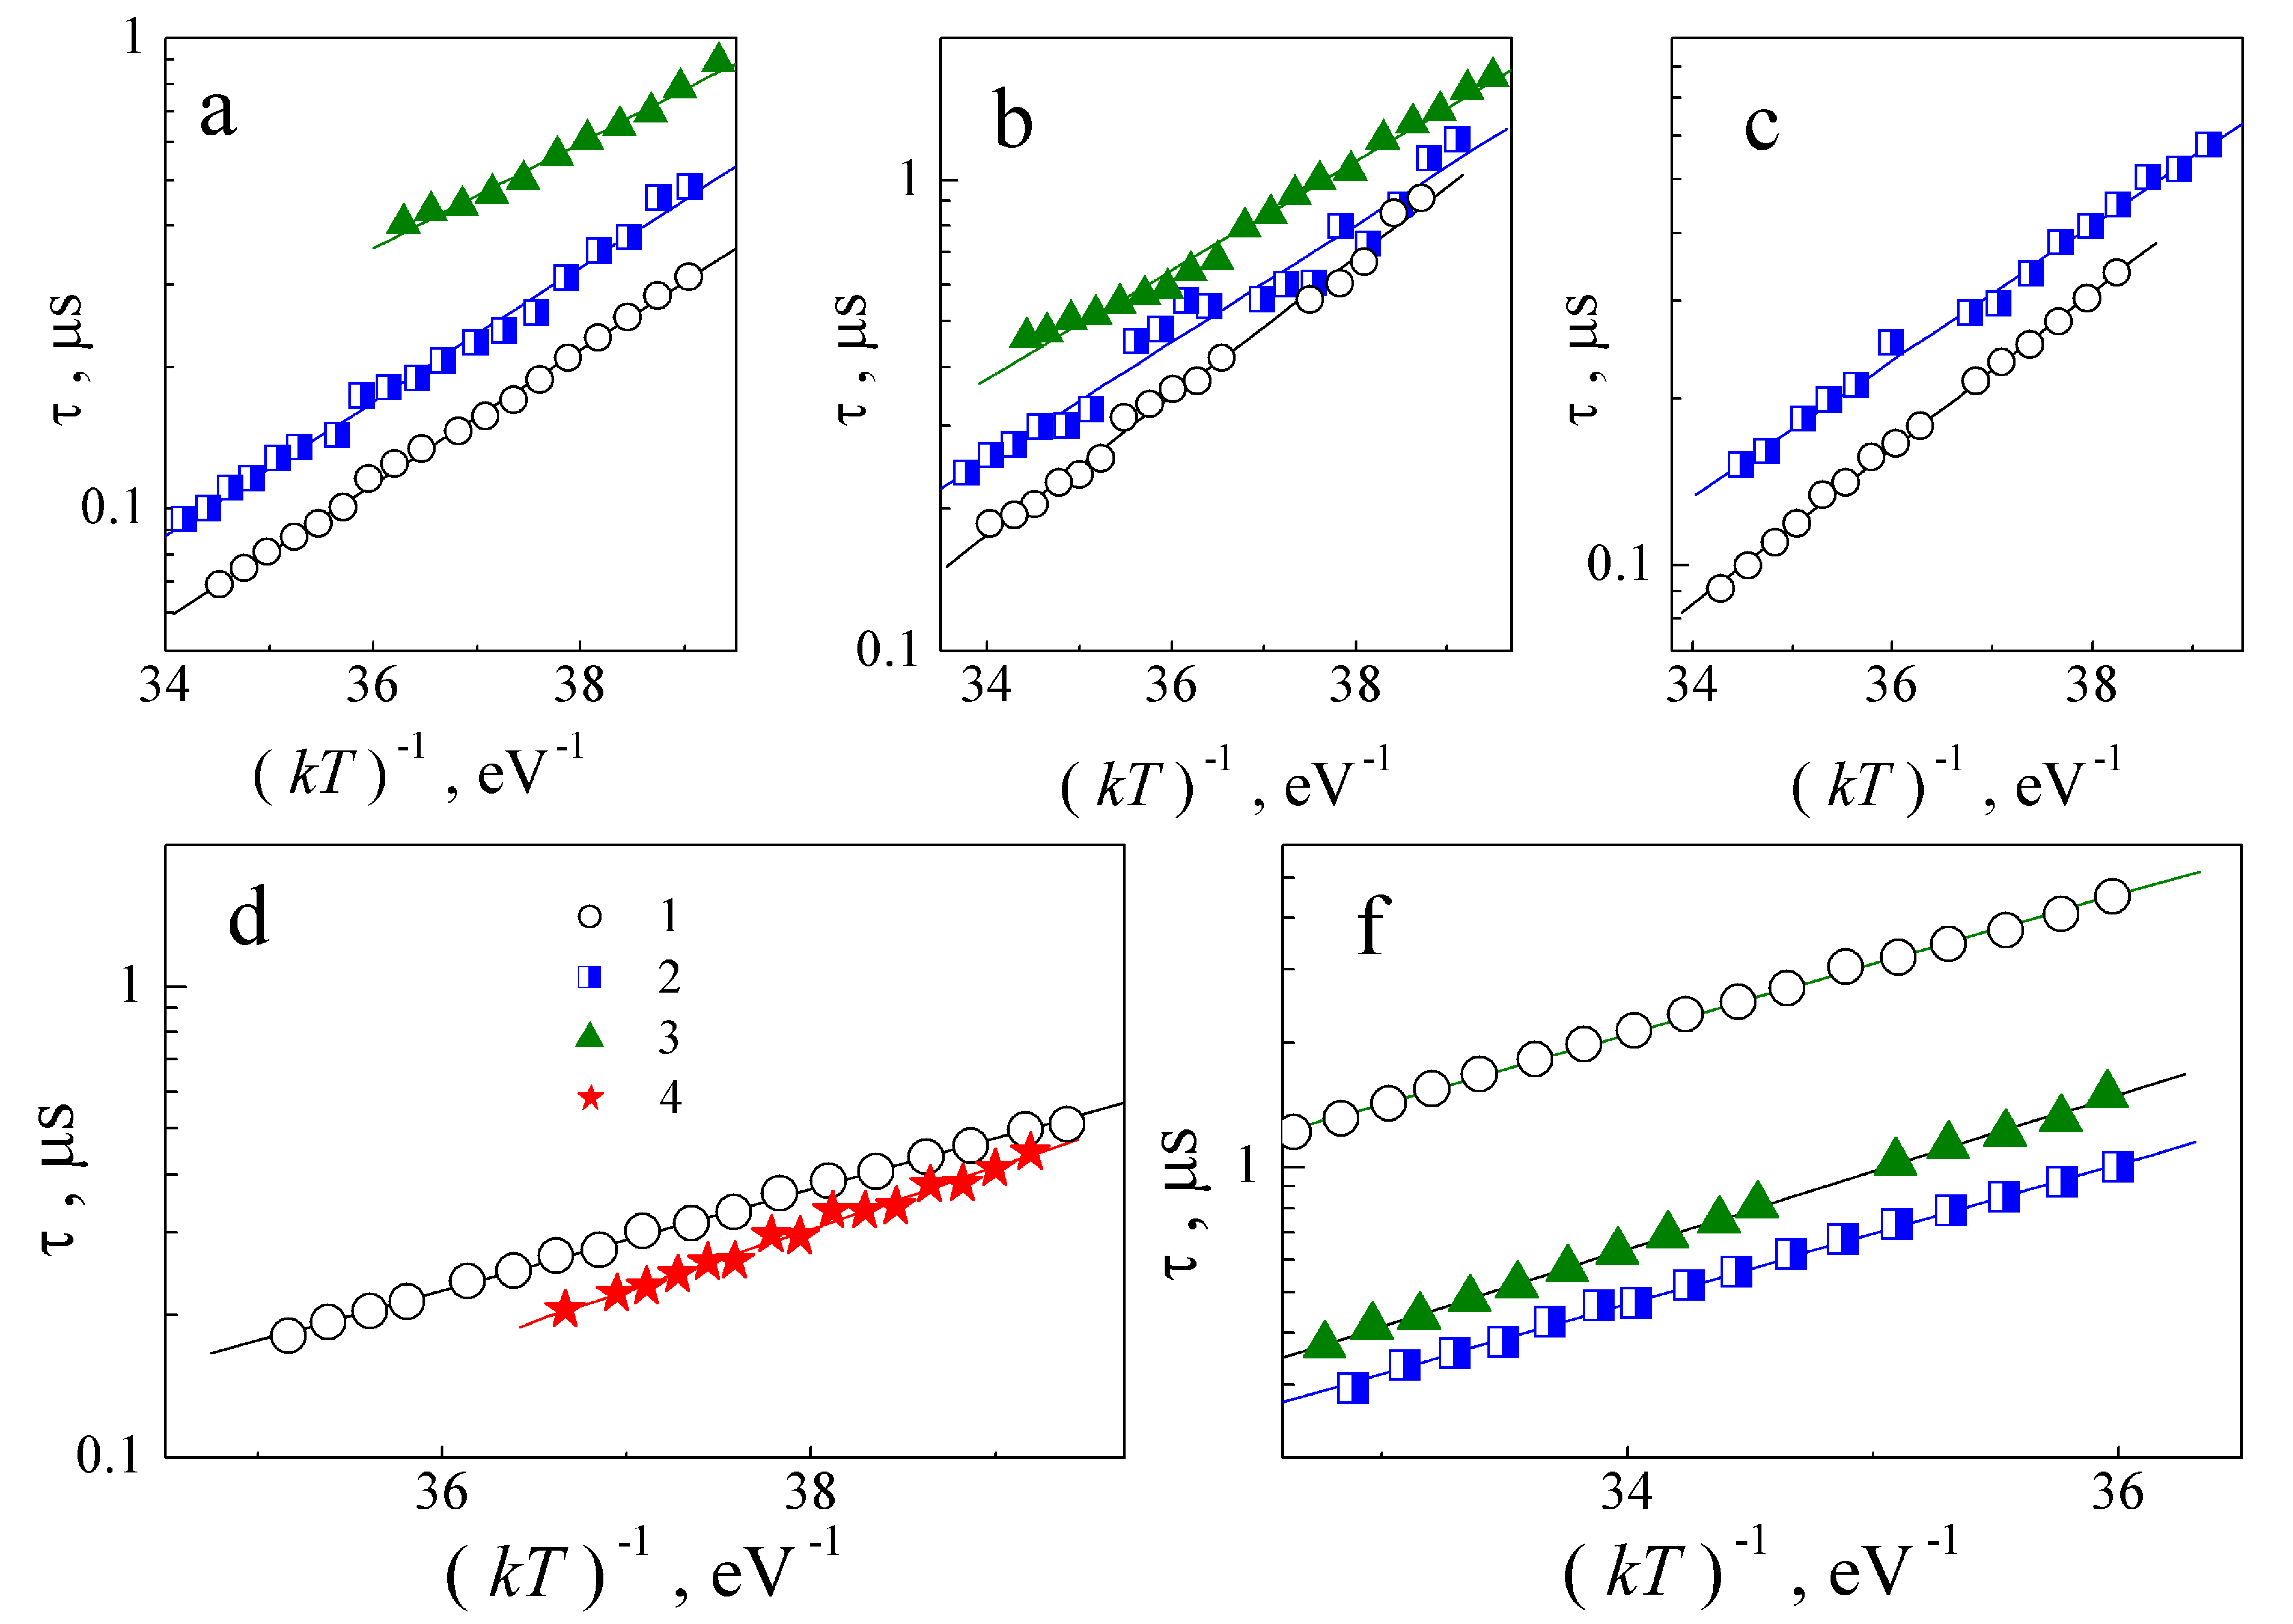
\includegraphics[width=0.7\textwidth]{Fig3}
\caption{\label{figTauTAV}
Dependences of TAV relaxation time on inverse temperature for samples SIC2 (a), SIC3 (b), GAS2 (c), GAE2 (d) and GAB1 (e) before and after MWT.
$t_\mathtt{MWT}$, s: 0 (curves 1), 20 (2), 40 (3), 60 (4)
}%
\end{figure*}



\begin{table*}
\caption{\label{tabMW}
The determined defect parameters in samples $n$--GaAs and $n$--6$H$--SiC
}
\begin{indented}
\item[]\begin{tabular}{@{}*{7}{c}}
\br
Sample& $t_{\rm MWT}$, s &Level &$(E_c-E_t)$, eV &$\sigma_n$, cm$^2$ $^{\rm a}$&$R_\mathrm{cur}$, m&$\xi_\mathrm{cur}$\\
\mr
SIC1& 0 &ESC1& $0.33\pm0.01$ &$(7\pm4)\cdot10^{-18}$&$\infty$&0\\ %\cline{2-7}
& 20 &ESC1& $0.33\pm0.01$ &$(5\pm3)\cdot10^{-19}$&170.2&$8.7\cdot10^{-7}$\\ %\cline{2-7}
& 40 &ESC2& $0.26\pm0.01$ &$(2\pm1)\cdot10^{-19}$&\multicolumn{2}{c}{\multirow{2}{*}{-}}\\ %\cline{2-5}
& 80 & \multicolumn{3}{c}{weak signal}&\multicolumn{2}{c}{}\\ %\hline
SIC2& 0 &ESC1& $0.33\pm0.01$ &$(7\pm4)\cdot10^{-18}$&$>2000$&$<1.2\cdot10^{-7}$\\ %\cline{2-7}
& 20 &ESC1& $0.33\pm0.01$ &$(5\pm3)\cdot10^{-19}$&171.9&$1.4\cdot10^{-6}$\\ %\hline
SIC3& 0 &ESC1& $0.34\pm0.02$ &$(3\pm2)\cdot10^{-18}$&3.8&$6.1\cdot10^{-5}$\\ %\cline{2-7}
& 20 &ESC2&$0.29\pm0.01$ &$(5\pm3)\cdot10^{-19}$&5.5&$4.2\cdot10^{-5}$\\ %\cline{2-7}
& 40 &ESC2& $0.26\pm0.01$ &$(10\pm7)\cdot10^{-20}$&\multicolumn{2}{c}{\multirow{2}{*}{-}}\\ %\cline{2-5}
& 80 &ESC2& $0.23\pm0.01$ &$(6\pm4)\cdot10^{-20}$&\multicolumn{2}{c}{}\\ %\hline
GAS1& 0 &EGA1& $0.32\pm0.02$ &$(3\pm2)\cdot10^{-17}$&-53.8&$-2.8\cdot10^{-6}$\\ %\cline{2-7}
& 20 &EGA1& $0.31\pm0.01$ &$(2\pm1)\cdot10^{-17}$&22.9&$6.5\cdot10^{-6}$\\ %\cline{2-7}
& 40 & \multicolumn{3}{c}{weak signal}&\multicolumn{2}{c}{-}\\ %\hline
GAS2& 0 &EGA1& $0.32\pm0.01$ &$(4\pm2)\cdot10^{-17}$&17.2&$8.7\cdot10^{-6}$\\ %\cline{2-7}
& 20 &EGA2& $0.28\pm0.01$ &$(5\pm2)\cdot10^{-18}$&14.7&$1.0\cdot10^{-5}$\\ %\cline{2-7}
& 40 & \multicolumn{3}{c}{weak signal}&\multicolumn{2}{c}{}\\ %\cline{1-5}
GAT& 0 &EGA3& $0.49\pm0.02$ &$(5\pm3)\cdot10^{-14}$&\multicolumn{2}{c}{}\\ %\cline{2-5}
& 20 &EGA4& $0.40\pm0.02$ &$(2\pm1)\cdot10^{-15}$&\multicolumn{2}{c}{}\\ %\cline{1-5}
GAE1& 0 &EGA5& $0.24\pm0.01$ &$(2\pm1)\cdot10^{-18}$&\multicolumn{2}{c}{}\\ %\cline{2-5}
& 60 &EGA2& $0.29\pm0.01$ &$(10\pm6)\cdot10^{-18}$&\multicolumn{2}{c}{}\\ %\cline{1-5}
GAE2& 0 &EGA5& $0.25\pm0.01$ &$(2\pm1)\cdot10^{-18}$&\multicolumn{2}{c}{}\\ %\cline{2-5}
& 60 &EGA2& $0.30\pm0.01$ &$(2\pm1)\cdot10^{-17}$&\multicolumn{2}{c}{}\\ %\cline{1-5}
GAE3& 0 &EGA6& $0.43\pm0.01$ &$(8\pm5)\cdot10^{-17}$&\multicolumn{2}{c}{-}\\ %\cline{2-5}
& 60 &EGA6& $0.46\pm0.02$ &$(7\pm4)\cdot10^{-16}$&\multicolumn{2}{c}{}\\ %\cline{1-5}
GAB1& 0 &EGA4& $0.39\pm0.01$ &$(10\pm7)\cdot10^{-18}$&\multicolumn{2}{c}{}\\ %\cline{2-5}
& 20 &EGA4& $0.39\pm0.01$ &$(4\pm2)\cdot10^{-17}$&\multicolumn{2}{c}{}\\ %\cline{2-5}
& 40 &EGA6& $0.43\pm0.02$ &$(10\pm6)\cdot10^{-17}$&\multicolumn{2}{c}{}\\ %\cline{1-5}
GAB2& 0 &EGA4& $0.40\pm0.01$ &$(10\pm6)\cdot10^{-17}$&\multicolumn{2}{c}{}\\ %\cline{2-5}
& 20 &EGA4& $0.41\pm0.01$ &$(10\pm6)\cdot10^{-17}$&\multicolumn{2}{c}{}\\ %\cline{2-5}
& 40 &EGA6& $0.45\pm0.02$ &$(4\pm2)\cdot10^{-16}$&\multicolumn{2}{c}{}\\  %\hline
\br
\end{tabular}
\item[] $^{\rm a}$ at $T=300$~K for SIC, GA, GAE and at $T=340$~K for GAB
\end{indented}
\end{table*}


\section*{References}

\bibliographystyle{iopart-num}
\bibliography{olikh}

\end{document}

